\section{Application II}
This section will demonstrate the section optimization of a simple 4-bay, 8-story steel frame using SAP2000 OAPI. Simulated annealing algorithm will be used for the optimization process, and the design will be performed according to the LRFD method.

\sidenote{
    
\qrcode[height=1in]{https://github.com/btayfur/structural-optimization/blob/main/Code/Examples/Exmp7/}}

\subsection{Steel frame model}
The model consists of a steel frame structure with 4 bays (5m span distance) and 8 stories (3m story height). Each floor has a uniformly distributed load of 40 kN/m over each span. All supports are modeled as fixed. Grade 36 steel is used throughout the structure. The unbraced length for beams is assumed to be 1/5 of the beam length. SAP2000 Steel Design tool will be used for design and optimization processes.

\begin{figure}[H]
    \centering
    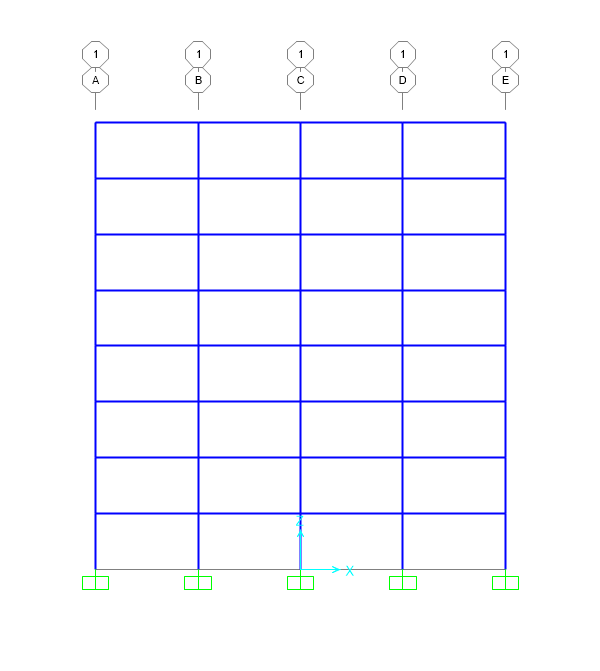
\includegraphics[width=0.8\textwidth]{weeks_new/imgs/exmp7_fig2.png}
    \caption{Steel frame model}
    \label{fig:model}
\end{figure}

\begin{figure}[H]
    \centering
    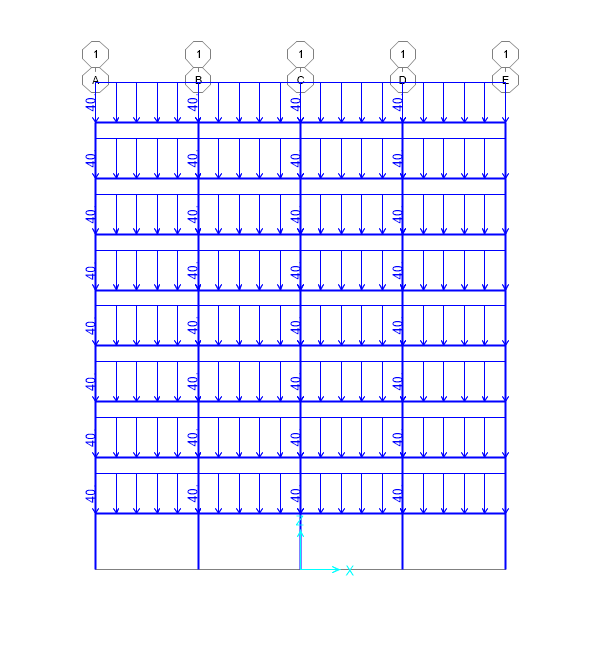
\includegraphics[width=0.8\textwidth]{weeks_new/imgs/exmp7_fig1.png}
    \caption{Loading Condition}
    \label{fig:loading}
\end{figure}

\begin{figure}[H]
    \centering
    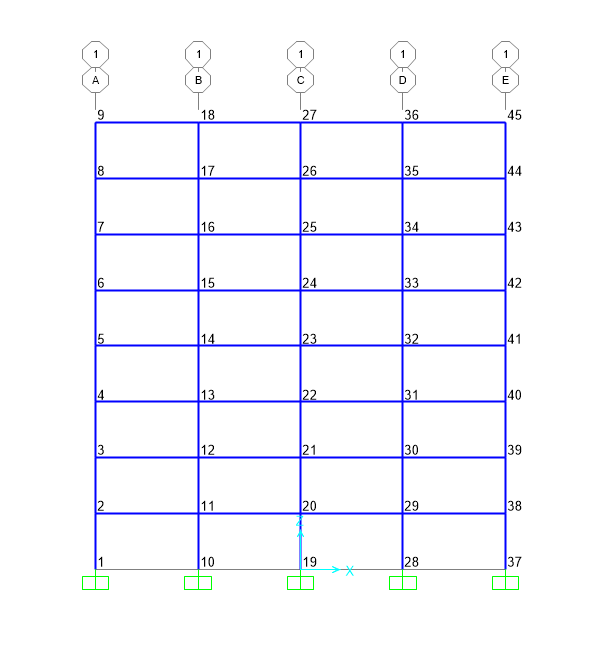
\includegraphics[width=0.8\textwidth]{weeks_new/imgs/exmp7_fig3.png}
    \caption{Numbering of joints}
    \label{fig:joints}
\end{figure}

\subsection{Section grouping}
Columns and beams in the structure are grouped to change every two floors. This results in a total of 4 column groups and 4 beam groups. Different section selections will be made for each group, and the sections of these groups will be optimized during the optimization process.

\subsubsection{Determination of selectable parameters}
The section list to be used in the optimization process consists of W profiles selected from the AISC catalog. The section list includes profiles in different sizes from W12 to W33. Appropriate section selection will be made from this list for each group, and the most suitable sections will be determined by the optimization algorithm.

\subsection{Optimization}

\subsubsection{Objective Function}
The objective function in the optimization process is set to minimize the total weight of the structure. This will provide both an economical solution and optimize the performance of the structure.
To calculate the structure weight, a "load case" named "weight" was created in the model. Since this load case does not contain any other forces, the sum of support reactions in the z-axis gives the weight of the structure. Additionally, as in many structural optimization problems, the objective function in this problem can be expressed as:

\begin{equation}
    f(x) = \sum_{i=1}^{n} \rho_i \cdot A_i \cdot L_i
\end{equation}
Here, $\rho_i$ represents the section weight, $A_i$ represents the section area, and $L_i$ represents the section length. \sidenote{
    In more complex problems using W sections, section naming can be utilized. For example, the $x35$ part of W12$\times$35 section indicates the weight per unit length. However, these values need to be converted to SI units.
}


\subsubsection{Constraints}
The following constraints are implemented using the SAP2000 Steel Design tool during the optimization process. The VerifyPassed() method returns the number of frame elements that do not meet the code requirements. In the background, all checks from buckling length to general interaction equations are performed. However, in many optimization studies—especially those that do not use OAPI and similar tools for speed—the following combined effect equations are used for verification:
\begin{equation}
    \frac{P_u}{\phi_c P_n} \geq 0.2; \quad c_1=\frac{P_u}{\phi_c P_n} + \frac{8}{9} \left(\frac{M_{ux}}{\phi_b M_{nx}} + \frac{M_{uy}}{\phi_b M_{ny}}\right) 
\end{equation}
\begin{equation}
    \frac{P_u}{\phi_c P_n} < 0.2; \quad c_2=\frac{P_u}{\phi_c P_n} +  \left(\frac{M_{ux}}{\phi_b M_{nx}} + \frac{M_{uy}}{\phi_b M_{ny}}\right) 
\end{equation}
\begin{equation}
    \forall i: c_i \leq 1.0
\end{equation}

\subsection{Optimization Results}
As mentioned earlier, simulated annealing algorithm is a stochastic method. Therefore, it is natural to obtain different results in each run. However, in a research study, the consistency of the algorithm can generally be better understood by making a large number of runs to better evaluate the general performance of the algorithm. In this example, only one run with a low iteration limit will be performed, and the results will be examined. However, when sufficient analysis time is allowed, the code within the scope of the example can be easily modified in this context.

\begin{figure}[H]
    \centering
    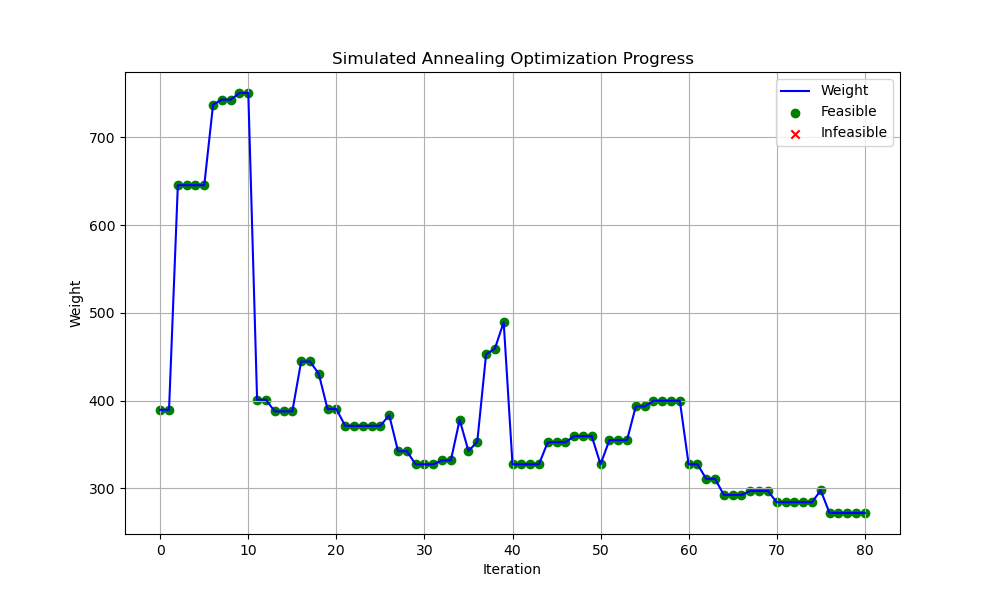
\includegraphics[width=0.8\textwidth]{weeks_new/imgs/exmp7_fig4.png}
    \caption{Change in structure weight during optimization}
    \label{fig:weight_change}
\end{figure}

\begin{table}
    \caption{Beam and column sections}
\end{table}

\begin{figure}[H]
    \centering
    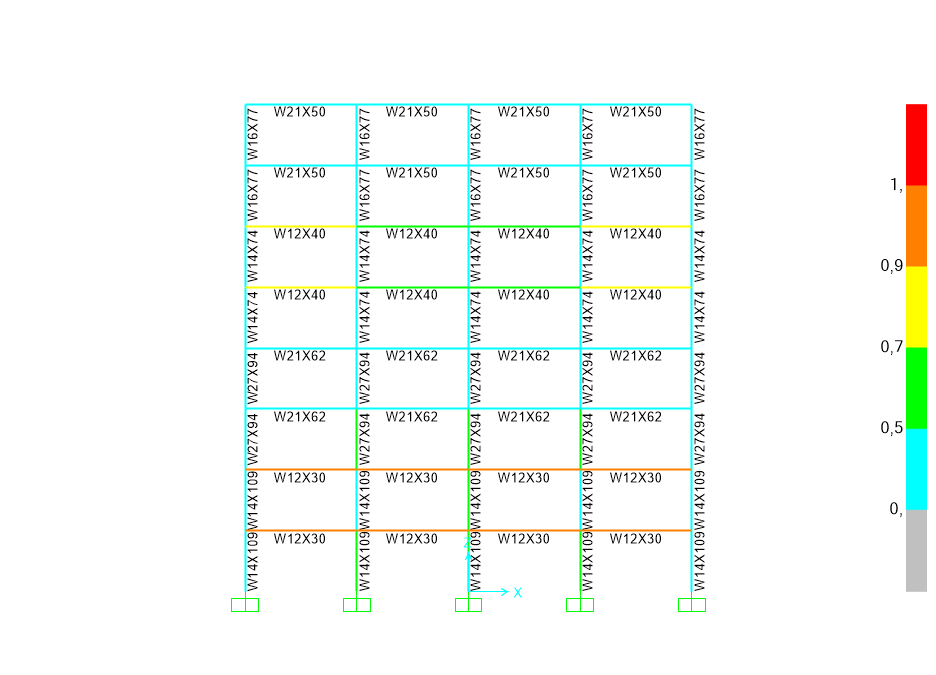
\includegraphics[width=0.8\textwidth]{weeks_new/imgs/exmp7_fig5.png}
    \caption{Demand/Capacity Ratio display of the optimal design}
    \label{fig:dcr_values}
\end{figure} 